%!TeX root = ./../MusterAbschlussarbeit.tex

%##########################################################
% Inhalt
%##########################################################

\clearpage
\chapter{Theoretische Grundlagen}
\section{Neuronale Netze}
Neuronale Netze (=NN) sind ein Modell für künstliche Intelligenz nach dem Vorbild des Gehirns. Sie bestehen aus mehreren Schichten verknüpfter Neuronen. Diese verarbeiten numerische Informationen und wandeln diese in einen Output.  In \ref{fig:künstlichesNeuron} ist der Aufbau eines künstlichen Neurons schematisch dargestellt. Jedes Neuron besitzt eine Aktivierungsfunktion, welche entscheidet, ob es aktiv ist oder nicht. Neuronen geben Werte von 0 (passiv) bis 1 (aktiv) als Output weiter. 

Um ein NN zu erzeugen, wird eine Vielzahl der Neuronen miteinander verknüpft. Die Ausgänge der vorderen Neuronen sind dabei immer mit den Eingängen der Neuronen der nächsten Schicht verknüpft. \ref{fig:neuronalesNetz} zeigt den Aufbau eines solchen Netzes. 

Wird ein NN initialisiert, werden Kantengewichte zwischen den Neuronen zufällig verteilt. Diese Kantengewichte entscheiden, wie stark einzelne Neuronen in die nachfolgende Rechnung eingehen.
Deshalb liefern untrainierte NN schlechte Ergebnisse und müssen lernen die Problemstellung richtig zu lösen. Dieser Prozess wird als Training bezeichnet.
Während des Trainings eines NN werden Kantengewichte angepasst, um die Heuristik  an ein optimales Ergebnis anzupassen. Richtig trainierte NN können gute Antworten für komplexe Problemstellungen geben, so liefern sie beispielsweise in der Mustererkennung gute Ergebnisse.\cite{lorenz_reinforcement_2020}
Für das Training von NN wird viel Rechenleistung gebraucht, da der Prozess mit vielen Rechenoperationen verbunden ist.
\cite{ertel_grundkurs_2021}

\begin{figure}[!htb]
	\centering
	\includegraphics[width=0.5\textwidth]{Bilder/künstlichesNeuron.png}
	\caption{Aufbau eines künstlichen Neurons \cite{noauthor_kunstliche_nodate}}
    \label{fig:künstlichesNeuron}
\end{figure}

\begin{figure}[!htb]
	\centering
	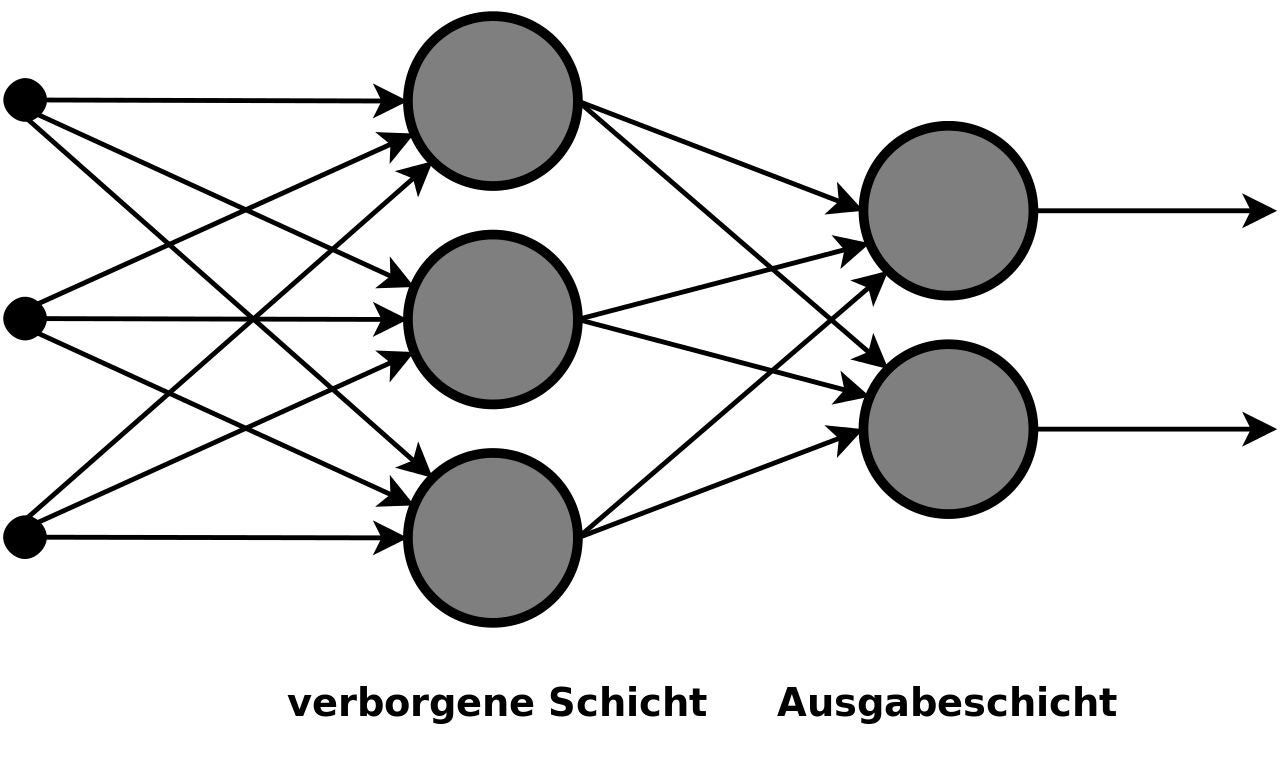
\includegraphics[width=0.5\textwidth]{Bilder/AufbauNN.png}
	\caption{Schematische Darstellung eines neuronalen Netzes \cite{noauthor_kunstliche_nodate}}
    \label{fig:neuronalesNetz}
\end{figure}



\clearpage
\section{Reinforcement Learning}
Reinforcement Learning ist ein Bereich des maschinellen Lernens, bei welchem ein Agent durch Interaktion mit seiner Umgebung (Environment) lernt, welche Aktionen in welchen Situationen am besten geeignet sind, um ein bestimmtes Ziel zu erreichen. Da ein Agent keine konkrete Vorgehensweise besitzt, versucht er über Trial-and-Error herrauszufinden welche Aktionen zu Belohnungen führen. \\
Bestandteile des RL sind der Agent und die Umwelt. Der Agent bekommt die Informationen der Umwelt übergeben und entscheidet welche Handlungen daraus folgen sollen. Das Environment setzt die Aktionen des Agenten in Handlungen (Aktionen) um und bewertet diese mit numerischen Belohnungen (Rewards). Anhand der erhaltenen Rewards, versucht der Agent seine Aktionen anzupassen, um die zukünftigen Belohnungen zu maximieren. \\
Ein RL-Agent nimmt seine Umgebung als eine Menge an bestimmten Zuständen wahr.
Jeder Zustand enthält eine Vielzahl von Merkmalen, welche für die Entscheidungsfindung relevant sein können.
Als Zustandsraum wird die Menge aller möglichen Zustände bezeichnet.\\
Auf jedem dieser Zustände ist es möglich eine bestimmte Menge an Aktionen auszuführen, welche das Umfeld in einen anderen Zustand überführen.
Die Menge aller möglichen Aktionen wird als Aktionsraum bezeichnet.\\
Wird eine Aktion auf einem bestimmten Zustand ausgeführt, so bezeichnet man die Zustandsübergänge bei Ausführung der Aktion als Zustandsübergangsfunktion.\\
Die Verhaltensstrategie  eines Agenten liefert zu jedem Zustand eine Aktion. Die Policy wird im Verlauf des Trainings erlernt.\\
Das Erlernen einer Policy erfolgt durch Training des Neuronalen Netzes. Zu Beginn des Trainings werden Kantengewichte des zur trainierenden Neuronalen Netzes zufällig verteilt. Um zu überprüfen ob seine Aktionen gut oder schlecht sind, erhält der Agent einen numerischen Rückgabewert, welcher jene Information beinhaltet. Diese numerischen Rückgabewerte werden als Belohnungen (Rewards) bezeichnet. Belohnungen werden vom Zustandsraum verteilt und können gutes Verhalten des Agenten durch positive Rewards und falsches Verhalten durch negative Rewards bestärken.
Der Agent versucht den Wert der erhaltenen Belohnungen zu maximieren und erlernt auf diese Weise eine optimale Policy. \\
\newpage
Probleme, welche beim RL auftreten können, sind unter anderem:  
\begin{itemize}
    \item Überanpassung 
    \item Belohnungsumgehung, 
    \item Sparse Rewards
    \item große Beobachtungsvektoren
\end{itemize}
Von \textbf{Überanpassung} spricht man, wenn der Agent ein Problem gut in der Lernumgebung, in welcher er trainiert wurde, lösen kann, allerdings nicht auf abweichenden Umgebungen. Es tritt auf, wenn der Agent zu spezialisiert auf seine Trainingsumgebung ist und sich nicht an andere Situationen anpassen kann. Diese Problem lässt sich durch Generalisierung des Trainingsprozesses beheben. Ein Agent, welcher in vielen zufällig generierten Umgebungen trainiert, kann deutlich besser mit neuen Situationen umgehen, benötigt im Gegenzug dazu auch mehr Zeit zum Trainieren. \cite{zhang_study_2018} \\
\textbf{Belohnungsumgehung} tritt auf, wenn der Agent lernt die Belohnungsfunktion zu manipulieren, um erhaltene Belohnungen zu maximieren, ohne das eigentliche Ziel der Aufgabe zu erreichen. Dies führt zu unerwünschtem Verhalten des Agenten. Verhindert werden kann dieses Problem, indem Belohnungen direkt mit dem Ziel verknüpft werden, also nur Belohnugnen ausgelöst werden, wenn tatsächlich positive Aktionen ausgeführt werden. \cite{pan_effects_2022} \\
Von \textbf{Sparse Rewards} spricht man, wenn die Lernumgebung dem Agenten nur selten oder unregelmäßig Belohnungen vergibt. Dies führt dazu, dass der Agent Schwierigkeiten hat, die ihm gegebene Aufgabe richtig zu erlernen. Um dieses Problem zu umgehen, kann man zusätzliche künstliche Belohnungen einführen, welche den Agenten auf den Weg zum richtigen Verhalten führen. Dies kann im Rückschluss jedoch wieder zur Belohnungsumgehung führen, wenn der Agent die Zwischenbelohnungen, nutzt um maximale Belohnungen zu erhalten. \cite{hare_dealing_2019} \\
Auch ein zu \textbf{großer Beobachtungsvektor} kann zu Komplikationen führen. Wird dem Agenten eine Vielzahl an Observationen zugeführt, müssen erheblich mehr Parameter im Modell verarbeitet werden, was zu größerem Berechnungsaufwand führt. Dadurch wird auch die Lerngeschwindigkeit verlangsamt und der Bedarf an Speicherplatz für die Modelle steigt. So ist es möglich, dass einfach erscheinende Aufgaben mehrere Tage an Rechenzeit benötigen, um ein gutes Modell zu generieren.
\cite{zai_einstieg_2020}

\newpage
\subsection{Markov Entscheidungsprozess}
Jedes RL Problem lässt sich durch den Markov Entscheidungsprozess (= MDP) beschreiben.
Der MDP ist ein mathematisches Modell für Entscheidungsprobleme, bei welchem der Agent abhängig von der Umwelt Entscheidungen trifft, um ein bestimmtes Ziel zu erreichen.
MDP setzen die Einhaltung der Markov-Eigenschaft vorraus. Diese ist erfüllt, wenn ein Zustandsübergang nur vom letzten Zustand und der letzten Aktion abhängig ist.
Hauptkomponenten des MDP sind eine endliche Menge valider Zustände, eine endliche Menge valider Aktionen, Belohnungsfunktion und Verhaltensstrategie.
Das Ziel eines MDP ist es eine optimale Policy, durch Maximierung der erhaltenen Belohnungen, zu ermitteln. \\
\ref{fig:markov} stellt den Ablauf eines MDP dar. Zu Beginn einer Episode befindet sich die Lernumgebung in einem gewissen Zustand. Dieser Zustand wird dem Agenten übergeben. Anhand der Beobachtungen führt der Agent eine Aktion aus, welche die Umgebung verändert. Die Veränderung der Umgebung erzeugt einen neuen Zustand, welcher im nächsten Schritt wiederum dem Agenten übergeben wird. Durch Auslösen von Aktionen in der Lernumgebung werden Belohnungen erzeugt, welche dem Agenten einen numerischen Wert liefern, ob die Aktion gut oder schlecht war. Der Agent versucht die erhaltenen Belohnungen zu maximieren.
Eine hohe Belohnung impliziert das richtige Verhalten zum Lösen des Problems, welches der Agent bewältigen muss.
Dieser Prozess wiederholt sich, bis das Problem gelöst wurde. \cite{zai_einstieg_2020}

\begin{figure}[!h]
	\centering
	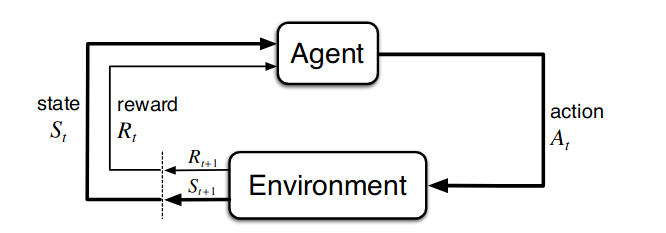
\includegraphics[width=0.7\textwidth]{Bilder/Markov.png}
	\caption{Ablauf eines MDP \cite{sutton_reinforcement_2014}}
	\label{fig:markov}
\end{figure}

\newpage
\section{Das Würfelspiel: Noch Mal}
Im modellierten Spiel 'Noch Mal!' geht es darum so viele Kästchen wie möglich anzukreuzen und damit viele Spalten und gleichfarbige Kästchen auszufüllen. Jeweils ein Farb- und ein Zahlenwürfel müssen kombiniert werden, um entsprechend verfügbare und zusammenhängende Felder der gewählten Farbe abzukreuzen. Dabei kann der Zahlenwürfel die Werte von eins bis fünf oder einen Zahlenjoker ergeben. Der Farbwürfel besitzt die fünf Farben des Feldes und einen Farbjoker. Gespielt wird nach folgenden Regeln:
\setlist{noitemsep}
\begin{enumerate}
    \item Felder in der Spalte H sind von Beginn an verfügbar
    \item Alle Kreuze müssen immer zusammenhängend in genau einem Farbblock der gewählten Farbe platziert werden
    \item Kreuze müssen waagerecht oder senkrecht benachbart zu einem bereits abgekreuzten Feld oder Teil der Spalte H sein, um verfügbar zu werden
    \item Es müssen genau so viele Felder angekreuzt werden, wie das Ergebnis des gewählten Zahlenwürfels
    \item Es könnte nicht mehr als 5 Kästchen in einem Zug abgekreuzt werden
    \item Wird ein Zahlenjoker gewählt, darf der Spieler eine Zahl von 1-5 bestimmen
    \item Wird ein Farbjoker gewählt, darf der Spieler eine Farbe bestimmen
\end{enumerate}

\begin{figure}[!h]
	\centering
	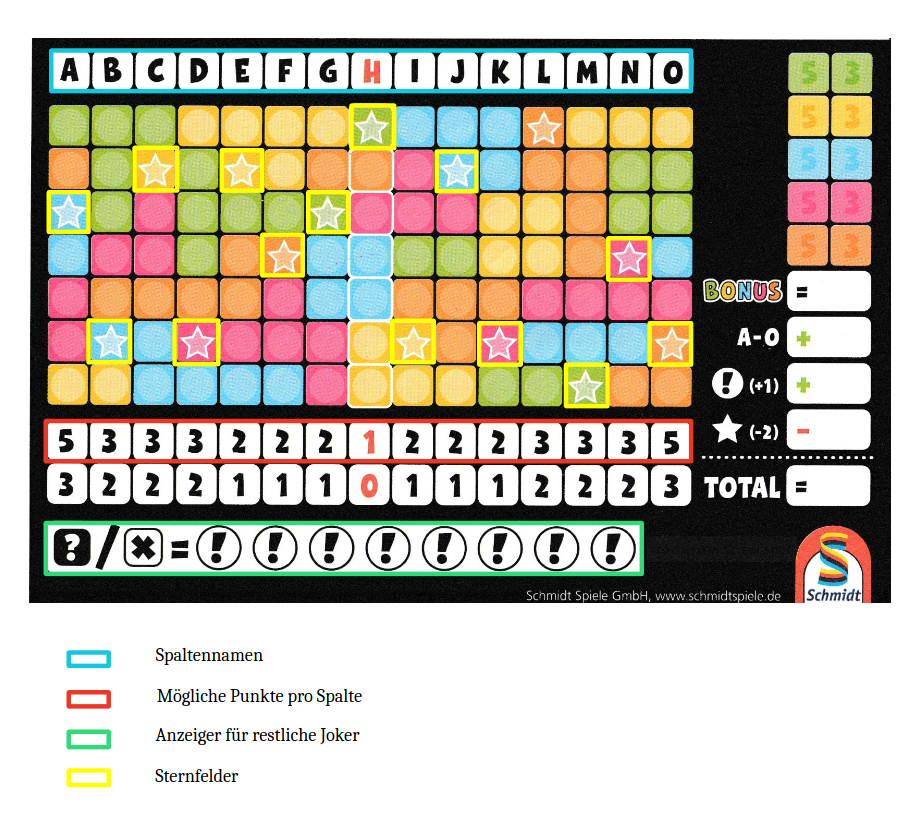
\includegraphics[width=0.7\textwidth]{Bilder/Abbildung2.png}
	\caption{Vorlage des schwarzen Spielfeldes mit Indikation der Punktewertung 
	\cite{schmidt_spiele_gmbh_spielregeln_nodate}}
	\label{fig:Vorlage}
\end{figure}

\begin{figure}[!h]
	\centering
	\includegraphics[width=0.7\textwidth]{Bilder/Beispielzüge.jpg}
	\caption{Beispiele für korrektes und falsches Ankreuzen aus der Spielanleitung 
	\cite{schmidt_spiele_gmbh_spielregeln_nodate}}
	\label{fig:Beispiel}
\end{figure}

Die Grafik \ref{fig:Vorlage} ist ein Spielfeld aus 'Noch mal!'. Nach Vorlage dieses Spielfelds wurde die Lernumgebung für den Agenten modelliert. Die blau markierten Felder geben den Spaltennamen der Spalten an. Die rot markierten Felder zeigen an, wie viele Punkte beim Ausfüllen der jeweiligen Spalte erzielt werden. Das grün markierte Feld zeigt die Anzahl der verbleibenden Joker an, wird ein Joker benutzt, muss eines der Felder abgestrichen werden. Zum Ende des Spiels erhält der Spieler Extrapunkte für die verbleibenden Joker. In jeder Spalte befindet sich ein gelb markiertes Sternfeld. Diese geben zum Ende des Spiels Minuspunkte, weshalb es wichtig ist alle Sternfelder auszufüllen. Abbildung \ref{fig:Beispiel} zeigt Beispiele für korrektes und fehlerhaftes Ankreuzen.


\clearpage


\subsection{Spielablauf Einspielervariante}
Der Spieler hat 30 Züge Zeit maximale Punkte zu erreichen und würfelt jede Spielrunde alle 4 Würfel, bestehend aus 2 Farb- und 2 Zahlenwürfeln. Anschließend wählt er ein Paar aus Farb- und Zahlenwürfel aus und kreuzt entsprechend des gewürfelten Paares verfügbare Felder auf dem Spielfeld ab.
Ein Spieler darf immer entscheiden, ob er Würfelwürfe zum Ankreuzen verwenden möchte oder nicht.
Um Kästchen anzukreuzen, wählt der Spieler eine Kombination aus Zahlen- und Farbwürfel aus. Wählt er beispielsweise 'Grün' und '2' so müssen 2 zusammenhängende grüne Felder angekreuzt werden. \\
Gelingt es dem  Spieler eine Spalte komplett auszufüllen, erhält er je nach Spalte Punkte dafür. Für äußere Spalten werden mehr Punkte vergeben als für die inneren Spalten.
Für das komplette Ausfüllen einer Farbe erhält der Spieler fünf Punkte pro ausgefüllter Farbe. Eine Farbe gilt als komplett ausgefüllt, wenn jedes Feld dieser Farbe abgekreuzt wurde.
Jedes nicht angekreuzte Sternfeld gibt zum Spielende zwei Minuspunkte.
Für jeden übrig gebliebenen Joker erhält der Spieler zum Ende des Spiels einen Punkt.\\
\ref{fig:Punkteübersicht} ist aus der Spielanleitung des Spiels. Sie zeigt an, wie viele Punkte erreichbar sind und bewertet das Ergebnis. Anhand dieser erreichten Punkte wird die Güte des Trainingsfortschritts bewertet.

\begin{figure}[!h]
	\centering
	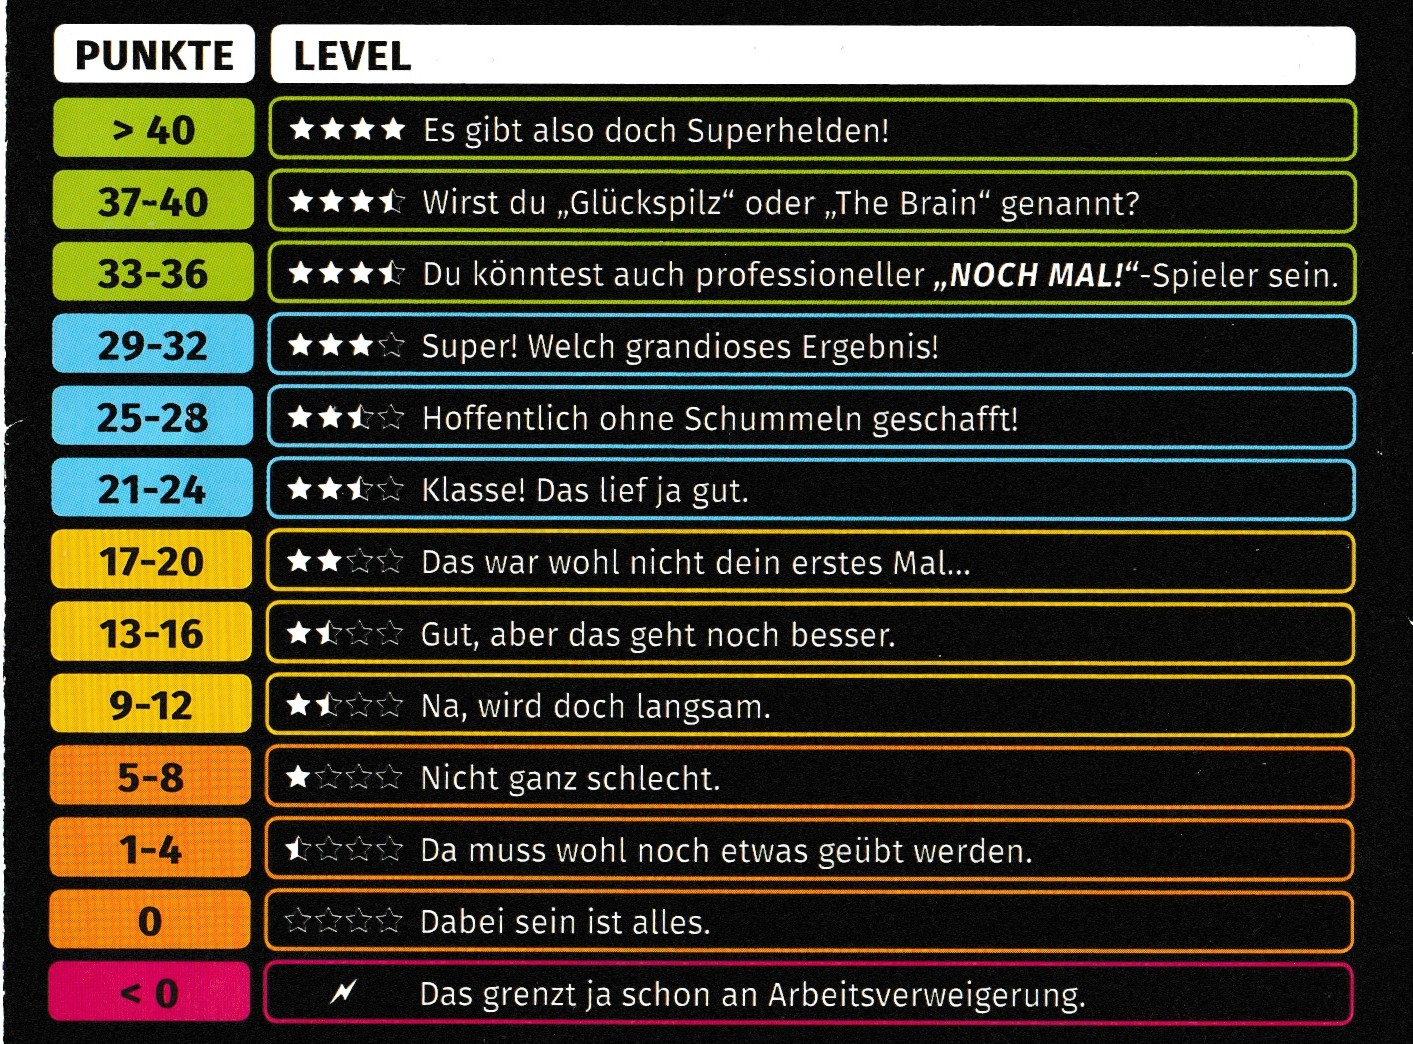
\includegraphics[width=0.5\textwidth]{Bilder/Punkte.jpeg}
	\caption{Grafik zur Bewertung der gesammelten Punkte der Einspieler Variante 
	\cite{schmidt_spiele_gmbh_spielregeln_nodate}}
	\label{fig:Punkteübersicht}
\end{figure}


\newpage 

Um im Spiel 'Noch mal' eine möglichst hohe Anzahl an Punkten zu erhalten, ist es wichtig nach folgenden Strategien zu spielen:\\
\textbf{Priorisierung äußerer Spalten}: Äußere Spalten geben mehr Punkte, weshalb es wichtig ist diese komplett auszufüllen. \\
\textbf{Beenden von Farben}: Vollständig ausgefüllte Farben geben viele Extrapunkte. Eine Farbe gilt als vollständig ausgefüllt, wenn kein Feld dieser Farbe mehr vorhanden ist. Im späten Spielverlauf kann es besser sein Farben komplett zu füllen anstatt Spalten zu werten. \\
 \textbf{Priorisieren von Sternfeldern}: Jedes ausgefüllte Sternfeld gibt 2 Punkte, eine gute Spielweise ist es so viele Sternfelder wie möglich auszufüllen. \\
\textbf{Strategische Nutzung von Jokern}: Ungenutzte Joker geben zum Ende des Spiels Punkte. Es ist gut diese so wenig wie möglich zu nutzen, um Extrapunkte zu bekommen. Jedoch können mit Hilfe von Jokern einfach bestimmte Felder gewählt werden, welche benötigt werden, um eine Wertung zu erzielen. 
